
\documentclass[aspectratio=169]{beamer}

%\setbeameroption{hide notes}
%\setbeameroption{show notes}
%\setbeameroption{show only notes}

  % Copyright (C) 2012 - EDF R&D - Michael Baudin

% To highlight source code
\usepackage{listings}
\definecolor{darkgreen}{rgb}{0,0.5,0}
\definecolor{violet}{rgb}{0.5,0,1}

% \usepackage{lmodern}% http://ctan.org/pkg/lm

\usetheme{Darmstadt} % http://tex.stackexchange.com/questions/177042/beamer-latex-customized-formats

\useoutertheme[subsection=false,footline=authortitle]{miniframes}
% RGB scaled on 0-255 scale (section 17.1.1), colors pulled from title block
\usecolortheme[RGB={44, 131, 82}]{structure}

% hide header:
\setbeamertemplate{headline}{}

\usepackage[utf8]{inputenc}
\usepackage[T1]{fontenc}

%\usepackage[french]{babel}
%\uselanguage{French}
%\languagepath{French}

\def\bx{{\bf x}}
\def\RR{\mathbb{R}}

\newcommand{\pyvar}[1]{\texttt{#1}}

\def \ot {OpenTURNS}

\hypersetup{colorlinks=true}

\lstset{
  % general command to set parameter(s)
   %basicstyle=\footnotesize\ttfamily, %
   %basicstyle=\normalsize \ttfamily, %
   basicstyle=\scriptsize\ttfamily, %
   keywordstyle=\color{violet}\bfseries,%
   commentstyle=\color{darkgreen}\bfseries,%
   showspaces=false,%
   stringstyle=\color{red}\bfseries, 
   otherkeywords={Gumbel, TruncatedDistribution, LatentVariableModel, %
        SmoothedUniformFactory, Uniform, PythonFunction, ComposedDistribution, %
        StudentCopula, StudentCopulaFactory, RankSobolSensitivityAlgorithm, %
	   MonteCarlo, IntervalMesher, PointToFieldFunctionalChaosAlgorithm, FieldFunctionalChaosSobolIndices, HistogramFactory, %
	   Graph, BoxCoxFactory, CompositeProcess, WhittleFactory, ARMAFactory, %
	   Basis, TrendFactory, BoxCoxTransform, SpatialFunction, TimeSeries, %
	   WelchFactory, GreaterOrEqual, IndependentCopula, %
	   SystemFORM, UnionEvent, IntersectionEvent},
}

\usepackage{adjustbox}
\usepackage[normalem]{ulem}

\title[OpenTURNS]{OpenTURNS release highlights}

\author[OpenTURNS et al.]{J. Schueller (Phimeca)}

\date[]{User Day \#17, June 14th 2024, EDF Lab}

%%%%%%%%%%%%%%%%%%%%%%%%%%%%%%%%%%%%%%%%%%%%%%%%%%%%%%%%%%%%%%%%%%%%%%%%%%%%%

  \begin{document}

%%%%%%%%%%%%%%%%%%%%%%%%%%%%%%%%%%%%%%%%%%%%%%%%%%%%%%%%%%%%%%%%%%%%%%%%%%%%%

  \begin{frame}
  \titlepage

  \begin{columns}
  \begin{column}[t]{0.05\textwidth}
        \end{column}
  
    \column{0.10\textwidth}
  \begin{center}

\includegraphics[height=0.04\textheight]{figures/airbus-logo-3d-blue.png}
\end{center}

    \column{0.05\textwidth}
  \begin{center}

\includegraphics[height=0.09\textheight]{figures/logo-edf.jpg}
\end{center}

     \column{0.05\textwidth}
  \begin{center}

\includegraphics[height=0.09\textheight]{figures/imacs-logo.jpg}
\end{center}

    \column{0.10\textwidth}
  \begin{center}

\includegraphics[height=0.05\textheight]{figures/onera-logo.png}
\end{center}

    \column{0.15\textwidth}
  \begin{center}

\includegraphics[height=0.08\textheight]{figures/logo-phimeca.png}
\end{center}

\column{0.01\textwidth}

  \end{columns}

  \end{frame}

\begin{frame}
\frametitle{Overview}

New features since last year in releases:

\begin{itemize}
\item v1.22: fall 2023
\item v1.23: spring 2024
\end{itemize}

\end{frame}
  
%%%%%%%%%%%%%%%%%%%%%%%%%%%%%%%%%%%%%%%%%%%%%%%%%%%%%%%%%%%%%%%%%%%%%%%%%%%%%

\begin{frame}
\frametitle{Contents}
\tableofcontents
\end{frame}

%%%%%%%%%%%%%%%%%%%%%%%%%%%%%%%%%%%%%%%%%%%%%%%%%%%%%%%%%%%%%%%%%%%%%%%%%%%%%

\begin{frame}{Not about}

\begin{itemize}
\item TruncatedOverMesh
\item BoundaryMesher
\item UniformOrderStatistics
\item New GEV/GPD estimators
\end{itemize}

\end{frame}

%%%%%%%%%%%%%%%%%%%%%%%%%%%%%%%%%%%%%%%%%%%%%%%%%%%%%%%%%%%%%%%%%%%%%%%%%%%%%

\section{Probabilistic modelling}

\begin{frame}[containsverbatim]
\frametitle{New distribution: Student / t-Copula}

\begin{itemize}
\item StudentCopula(nu, R): The distribution
\item StudentCopulaFactory: Its estimator (xref "Interval Estimation for Bivariate t-Copulas via Kendall’s Tau")
\end{itemize}

\begin{figure}
   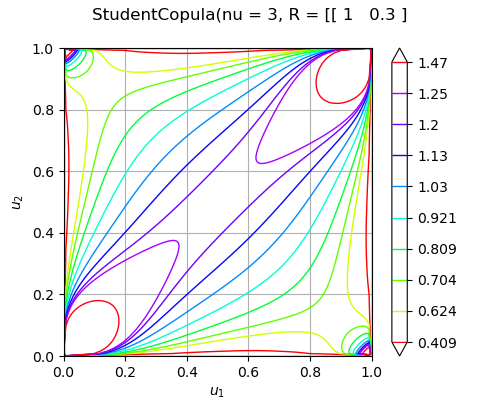
\includegraphics[height=0.5\textheight]{figures/StudentCopula}
   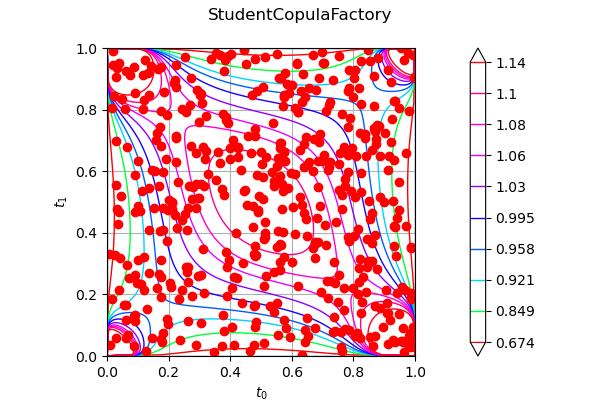
\includegraphics[height=0.5\textheight]{figures/StudentCopulaFactory}
\end{figure}

\begin{small}
\lstset{language=python}
\begin{lstlisting}
# OT < 1.23
R = ot.CorrelationMatrix(dim, [1.0, 0.5, 0.5, 1.0])
copula = ot.Student(3.5, [0.0] * 2, [1.0] * 2, R).getCopula()
\end{lstlisting}
\end{small}

\end{frame}

%%%%%%%%%%%%%%%%%%%%%%%%%%%%%%%%%%%%%%%%%%%%%%%%%%%%%%%%%%%%%%%%%%%%%%%%%%%%%

\begin{frame}[containsverbatim]
\frametitle{New distribution estimator for SmoothedUniform}

\begin{itemize}
\item Method of moments for initialization
\item Maximum likelihood for the final estimator
\end{itemize}

\begin{figure}
   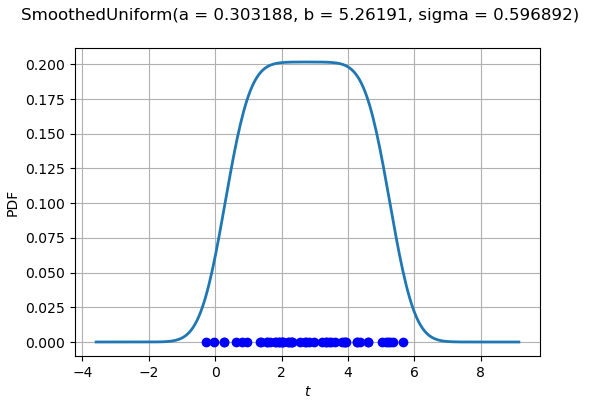
\includegraphics[width=0.4\textwidth]{figures/SmoothedUniformFactory}
\end{figure}

\begin{small}
\begin{lstlisting}
import openturns.experimental as otexp
estimated = otexp.SmoothedUniformFactory().build(sample)
\end{lstlisting}
\end{small}


\end{frame}

%%%%%%%%%%%%%%%%%%%%%%%%%%%%%%%%%%%%%%%%%%%%%%%%%%%%%%%%%%%%%%%%%%%%%%%%%%%%%

\begin{frame}[containsverbatim]
\frametitle{Latent variable model}

\begin{itemize}
\item Covariance model, for eg Kriging
\item Covariance between different unordered values (or levels) of a categorical variable
\item Parameters: coordinates in the latent space
\item Zhang2020: "A latent variable approach to Gaussian process modeling with qualitative and quantitative factors"
\end{itemize}

\vspace{30pt}

\begin{small}
\begin{lstlisting}
import openturns.experimental as otexp
covModel = otexp.LatentVariableModel(3, 2)
activeCoordinates = [0.1, 0.3, -0.4]
covModel.setLatentVariables(activeCoordinates)
\end{lstlisting}
\end{small}

\end{frame}

%%%%%%%%%%%%%%%%%%%%%%%%%%%%%%%%%%%%%%%%%%%%%%%%%%%%%%%%%%%%%%%%%%%%%%%%%%%%%

\section{Metamodelling}

\begin{frame}[containsverbatim]
\frametitle{New Field metamodeling capabilities}
\begin{itemize}
\item Vector to field metamodeling and sensitivity using KL + chaos
\end{itemize}

\begin{figure}
   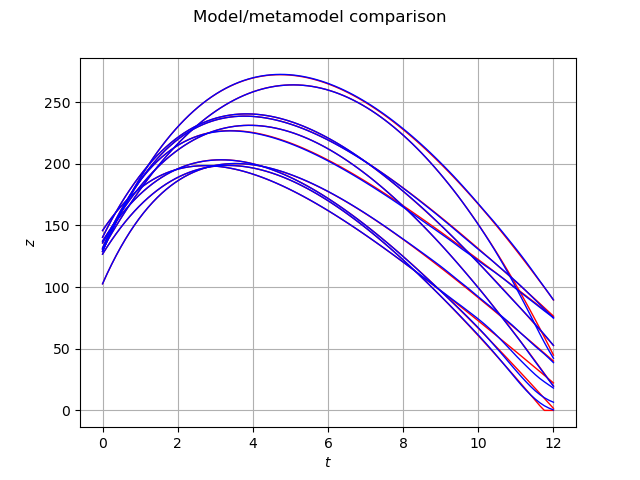
\includegraphics[width=0.3\textwidth]{figures/sphx_glr_plot_viscous_fall_metamodel_001}
   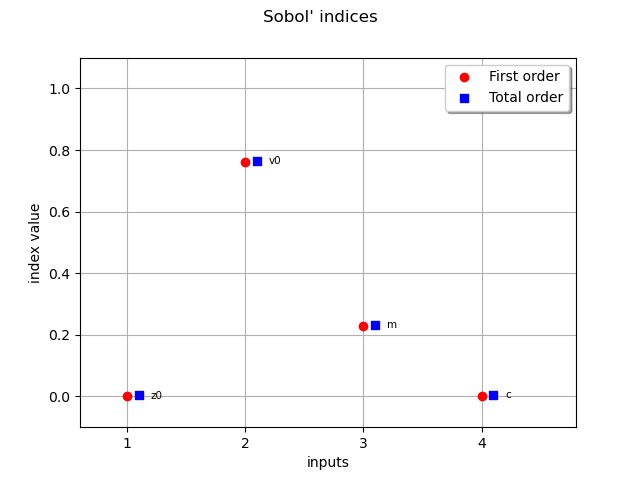
\includegraphics[width=0.3\textwidth]{figures/sphx_glr_plot_viscous_fall_metamodel_002}
   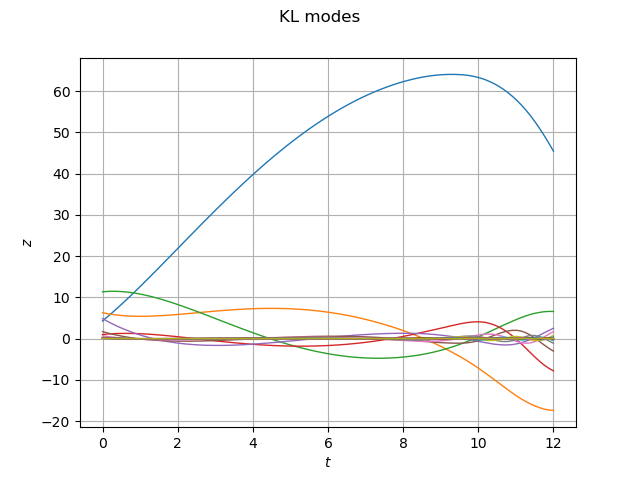
\includegraphics[width=0.3\textwidth]{figures/sphx_glr_plot_viscous_fall_metamodel_003}
\end{figure}

\begin{small}
\begin{lstlisting}
# metamodel
algo = otexp.PointToFieldFunctionalChaosAlgorithm(X, Y, distribution)
algo.run(); result = algo.getResult()
metaModel = result.getPointToFieldMetaModel()

# sensitivity
sensitivity = otexp.FieldFunctionalChaosSobolIndices(result)
s1 = sensitivity.getFirstOrderIndices()
st = sensitivity.getTotalOrderIndices()
\end{lstlisting}
\end{small}


\end{frame}



%%%%%%%%%%%%%%%%%%%%%%%%%%%%%%%%%%%%%%%%%%%%%%%%%%%%%%%%%%%%%%%%%%%%%%%%%%%%%

\section{Sensitivity}

\begin{frame}[containsverbatim]
\frametitle{Rank-based Sobol' indices}

\begin{itemize}
\item Data-driven (no need for dedicated design of experiments, just iid design)
\item Only first-order indices
\item Gamboa2022: "Global sensitivity analysis: A novel generation of mighty estimators based on rank statistics"
\end{itemize}

\begin{figure}
   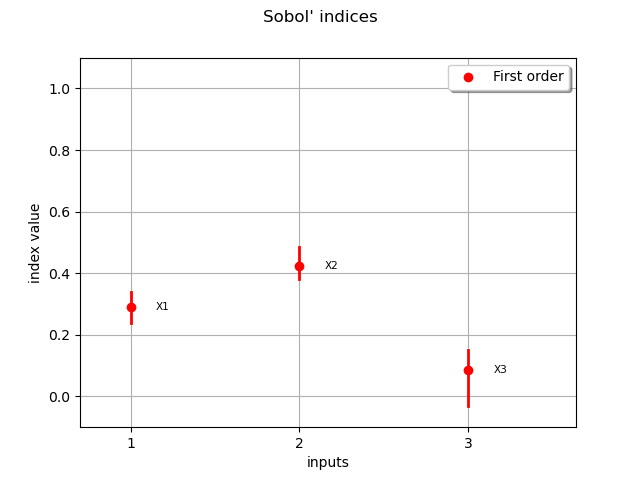
\includegraphics[width=0.3\textwidth]{figures/sphx_glr_plot_sensitivity_rank_sobol_001}
\end{figure}

\begin{small}
\begin{lstlisting}
X = distributionX.getSample(N)
Y = f(X)
algo = otexp.RankSobolSensitivityAlgorithm(X, Y)
s1 = algo.getFirstOrderIndices()
\end{lstlisting}
\end{small}

\end{frame}

%%%%%%%%%%%%%%%%%%%%%%%%%%%%%%%%%%%%%%%%%%%%%%%%%%%%%%%%%%%%%%%%%%%%%%%%%%%%%

\section{Misc}

\begin{frame}
\frametitle{Documentation improvements}
\begin{itemize}
\item Lots of new examples: chaos, cv, regression, MLE, functions, integration, enumerate, ...
\item New usecases: fire satellite, wing weight, Linthurst/Coles datasets
\end{itemize}

\begin{center}

\includegraphics[width=0.3\textwidth]{figures/stiffened_panel_simulation}
\end{center}

\begin{itemize}
\item Example minigalleries linking to relevant examples
\item Automatic checking of every internal links
\item Lot of time invested in the improvement of the documentation
\end{itemize}
\end{frame}

%%%%%%%%%%%%%%%%%%%%%%%%%%%%%%%%%%%%%%%%%%%%%%%%%%%%%%%%%%%%%%%%%%%%%%%%%%%%%

\begin{frame}
\frametitle{Other improvements}
\begin{itemize}
\item Multidimensional integration using cuba library (CubaIntegration)
\item New class for integration from an existing design of experiment (ExperimentIntegration)
\item Faster KDTree implementation using nanoflann library
\item Faster TruncatedDistribution with n-d CDF inversion
\end{itemize}

\vspace{6pt}

\begin{center}

\includegraphics[width=0.15\textwidth]{figures/bugfix}
\end{center}

\end{frame}

%%%%%%%%%%%%%%%%%%%%%%%%%%%%%%%%%%%%%%%%%%%%%%%%%%%%%%%%%%%%%%%%%%%%%%%%%%%

\begin{frame}
\frametitle{Packaging 1/2}
\begin{block}{Python channels}
\begin{itemize}
\item Pip (and uv), Conda
\item Versions: 3.8-3.12
\item OS: Windows, Linux, MacOS
\item Architectures: x86\_64, arm64 (MacOS-only)
\end{itemize}
\end{block}

\begin{figure}
   
\includegraphics[width=0.3\textwidth]{figures/PyPI_logo}
   
\includegraphics[width=0.3\textwidth]{figures/Conda_logo.svg}
\end{figure}

\end{frame}

\begin{frame}
\frametitle{Packaging 2/2}
\begin{block}{Supported Linux distributions}
\begin{itemize}
\item Ubuntu 22/24
\item Debian 11/12
\item Fedora 39/40
\item CentOS 8
\item OpenSUSE 15.5/15.6
\item Mageia 8
\item ArchLinux
\end{itemize}

... and FreeBSD

\end{block}


\begin{center}

\includegraphics[width=0.05\textwidth]{figures/debian-openlogo-100}

\includegraphics[width=0.08\textwidth]{figures/ubuntu}

\includegraphics[width=0.08\textwidth]{figures/Fedora-Logo}

\includegraphics[width=0.08\textwidth]{figures/centos-logo}

\includegraphics[width=0.08\textwidth]{figures/opensuse-logo}

\includegraphics[width=0.15\textwidth]{figures/200px-Logo_mageia_official}

\includegraphics[width=0.15\textwidth]{figures/archlinux-logo}

\includegraphics[width=0.15\textwidth]{figures/FREEBSD_Logo_Horiz_Pos_RGB}
\end{center}

\end{frame}

%%%%%%%%%%%%%%%%%%%%%%%%%%%%%%%%%%%%%%%%%%%%%%%%%%%%%%%%%%%%%%%%%%%%%%%%%%%

\begin{frame}
\frametitle{Outlook}
\begin{block}{2024-2025 work}
\begin{itemize}
\item Conditional distributions / Bayesian
\item Quantiles estimation / tolerance intervals
\item Calibration (functional models, bound constraints)
\item New GPR API
\item LOLA-Voronoi sequential design
\item Cross-validation of functional chaos expansion
\end{itemize}
\end{block}
\end{frame}

%%%%%%%%%%%%%%%%%%%%%%%%%%%%%%%%%%%%%%%%%%%%%%%%%%%%%%%%%%%%%%%%%%%%%%%%%%%%%

\begin{frame}
\frametitle{END}

Thank you for your attention!

Any questions?

\begin{center}
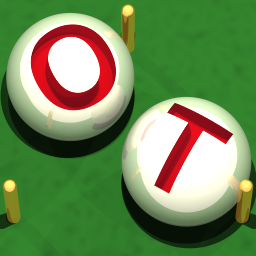
\includegraphics[width=0.2\textwidth]{figures/logo-ot-small}
\end{center}

\end{frame}

% %%%%%%%%%%%%%%%%%%%%%%%%%%%%%%%%%%%%%%%%%%%%%%%%%%%%%%%%%%%%%%%%%%%%%%%%%%%%%
% 
% \section{Bibliography}
% 
% \begin{frame}
% \frametitle{Bibliography}
% 
% \begin{itemize}
% \item Airbus, EDF, ONERA, Phimeca Engineering, IMACS.
% OpenTURNS, a scientific library usable as a Python module dedicated to the treatment of uncertainties, 
% \url{www.openturns.org}.
% \item Airbus, EDF, Phimeca Engineering, IMACS. Documentation of OpenTURNS, version 1.9. 
% \url{http://openturns.github.io/openturns/1.9/contents.html}
% \item  Michaël Baudin, Anne Dutfoy, Bertrand Iooss, and Anne-Laure Popelin. 
% OpenTURNS: An Industrial Software for Uncertainty Quantification in Simulation, 
% Handbook of Uncertainty Quantification, 
% pages 1-38. Springer International Publishing, 2016
% \end{itemize}
% 
% \end{frame}

\end{document}
